\documentclass[11pt,landscape,a4paper]{article}
\newcommand\hmmax{0}
\newcommand\bmmax{0}
\usepackage[utf8]{inputenc}
\usepackage[ngerman]{babel}
\usepackage{amsmath, bm}
\usepackage{bbm}
\usepackage{tikz}
\usetikzlibrary{shapes,positioning,arrows,fit,calc,graphs,graphs.standard}
\usepackage[nosf]{kpfonts}
\usepackage[t1]{sourcesanspro}
%\usepackage[lf]{MyriadPro}
%\usepackage[lf,minionint]{MinionPro}
\usepackage{multicol}
\usepackage{wrapfig}
\usepackage[top=0mm,bottom=4mm,left=0mm,right=1mm]{geometry}
% \usepackage[framemethod=tikz]{mdframed}
\usepackage{microtype}
\usepackage{mathptmx}
\usepackage{paralist}
\usepackage{algorithm}% http://ctan.org/pkg/algorithms
\usepackage{algpseudocode}% http://ctan.org/pkg/algorithmicx
\usepackage[framemethod=tikz]{mdframed}

\thinmuskip=3mu
\medmuskip=4mu %plus 2mu minus 4mu
\thickmuskip=5mu
\let\bar\overline

\definecolor{mygrey}{cmyk}{0,0,0,0.85}
\definecolor{myred}{cmyk}{0.81,0.81,0,0.3}
\DeclareMathOperator*{\argmin}{arg\,min}
\DeclareMathOperator*{\argmax}{arg\,max}

\newcommand{\E}[2][]{\mathbb{E}_{#1}[#2]}
\renewcommand{\P}[1]{\mathbb{P}(#1)}
\newcommand{\sampled}{\thicksim}
\newcommand{\Gt}{\theta}
\newcommand{\Ge}{\epsilon}
\newcommand{\Geb}{\mathbb{\epsilon}}
\newcommand{\Gth}{\hat{\theta}}
\newcommand{\Gts}{\theta^\star}
\newcommand{\Gb}{\beta}
\newcommand{\Gbb}{\mathbb{\beta}}
\newcommand{\convP}{\overset{p}{\to}}
\newcommand{\GNormal}{\mathcal{N}(\mu,\,\sigma^{2})}
\newcommand{\NNormal}{\mathcal{N}(0,\,1)}
\newcommand{\Normal}[2]{\mathcal{N}(#1,\,#2)}
\newcommand{\Var}{\mathrm{Var}}
\newcommand{\Cov}{\mathrm{Cov}}
\newcommand{\bx}{\mathbf{x}}
\newcommand{\bX}{\mathbf{X}}
\newcommand{\bzero}{\mathbf{0}}
\newcommand{\bY}{\mathbf{Y}}
\newcommand{\bb}{\mathbf{b}}
\newcommand{\Gbs}{\beta^\star}
\newcommand{\Data}{\mathcal{D}}
\newcommand{\Datatrain}{\mathcal{D}^{train}}
\newcommand{\Datatest}{\mathcal{D}^{test}}
\newcommand{\HypotesisSpace}{\mathcal{H}}
\newcommand{\Lossfct}{\mathcal{L}}
\newcommand{\Midentity}[1]{\mathbb{I}_{#1}}
\newcommand{\R}[1][]{\mathbb{R}^{#1}}

\DeclareMathOperator{\di}{d\!}

% Reset weird mathptmx \mathcal symbols
\DeclareMathAlphabet{\mathcal}{OMS}{cmsy}{m}{n}

% Hackeroni for smaller syms
\newcommand{\smallsim}{\smallsym{\mathrel}{\sim}}

\makeatletter
\newcommand{\smallsym}[2]{#1{\mathpalette\make@small@sym{#2}}}
\newcommand{\make@small@sym}[2]{%
  \vcenter{\hbox{$\m@th\downgrade@style#1#2$}}%
}
\newcommand{\downgrade@style}[1]{%
  \ifx#1\displaystyle\scriptstyle\else
    \ifx#1\textstyle\scriptstyle\else
      \scriptscriptstyle
  \fi\fi
}
\makeatother
% End hackeroni

\pgfdeclarelayer{background}
\pgfsetlayers{background,main}

\everymath\expandafter{\the\everymath \color{mygrey}}
\everydisplay\expandafter{\the\everydisplay \color{mygrey}}

\renewcommand{\baselinestretch}{.75}
\pagestyle{empty}


\makeatletter
\renewcommand{\section}{\@startsection{section}{1}{0mm}%
                                {.2ex}%
                                {.2ex}%x
                                {\color{myred}\sffamily\small\bfseries}}

\renewcommand{\subsection}{\@startsection{subsection}{1}{0mm}%
                                {.2ex}%
                                {.2ex}%x
                                {\sffamily\bfseries}}


\makeatother
\setlength{\parindent}{0pt}
\setlength{\columnsep}{5pt}

\begin{document}
\small
\begin{multicols*}{5}
\fontdimen2\font=0.3ex
\section*{Background}
\textbf{Linear Algebra}\\
$\| \mathbf{x} \|_p = \left( \sum |x_i|^p \right)^{1/p}$ \quad $\| \mathbf{x} \|_\infty = \max |x_i|$  
$\text{tr} (\mathbf{A} \mathbf{x} \mathbf{x}^T) = \mathbf{x}^T \mathbf{A} \mathbf{x}$ \\ $| \mathbf{A} \mathbf{B} | = | \mathbf{A} | | \mathbf{B} |$ \quad
$| \mathbf{A}^m | = | \mathbf{A} |^m$ 
$(\mathbf{A} {+} \mathbf{U} \mathbf{C} \mathbf{V})^{\text{-}} {=} \mathbf{A}^{\text{-}} {-} \mathbf{A}^{\text{-}} \mathbf{U} (\mathbf{C}^{\text{-}} {+} \mathbf{V} \mathbf{A}^{\text{-}} \mathbf{U})^{\text{-}} \ \ \mathbf{V} \mathbf{A}^{\text{-}}$ \\
$(\mathbf{A} + \mathbf{B})^{-1} = \mathbf{A}^{-1} - \mathbf{A}^{-1} (\mathbf{A} + \mathbf{B})^{-1} \mathbf{A}^{-1}$ \\
$\mathbf{U} (\mathbf{V} \mathbf{U} + \mathbf{I})^{-1} = (\mathbf{U} \mathbf{V} + \mathbf{I})^{-1} \mathbf{U}$ \\
$\mathbf{I} - \mathbf{A} (\mathbf{I} + \mathbf{A})^{-1} = (\mathbf{I} + \mathbf{A})^{-1}$
\vspace{4px}\\
\textbf{Probability}\\
$\text{Ber}(x|\theta) = \theta^x(1-\theta)^{1-x} \quad 0 \leq \theta \leq 1$
$\mathbb{P}[X|Y]=\frac{\mathbb{P}[X,Y]}{\mathbb{P}[Y]}=\frac{\mathbb{P}[Y|X]\mathbb{P}[X]}{\mathbb{P}[Y]}$ \\
$p_{Y}(y) = p_{X}(g^{-1}(y)) \left| \det \frac{\partial g^{-1}(y)}{\partial y} \right|$
% \vspace{4px}\\
$\mathbbm{E}[X]=\int_{\Omega}xp(x)\di x=\int_{\omega}x\mathbb{P}[X{=}x]\di x$ \\
$\mathbb{E}_{Y|X}[Y]{=}\mathbb{E}_{Y}[Y|X]$ | $\mathbb{E}_{Y}[\mathbb{E}_{X}[X|Y]] {=} \mathbb{E}_{X}[X]$
$\mathbb{E}_{X,Y}[f(X,Y)]=\mathbb{E}_{X}\mathbb{E}_{Y|X}[f(X,Y)|X]$
% \vspace{4px} \\
$\mathbb{V}(X){=}\mathbb{E}[(X{-}\mathbb{E}[X])^2]{=}\mathbb{E}[X^2]{-}\mathbb{E}[X]^2$\\
$\text{Var}(X) {=} \mathbb{E}[\text{Var}(X \mid Y)] {+} \text{Var}(\mathbb{E}[X \mid Y])$  
$\mathbb{V}[X{+}Y]{=}\mathrm{Var}[X]{+}\mathrm{Var}[Y]{+}2\Cov(X, Y)$ \\
$\mathrm{Cov}(\bX ,\bY)=\E[]{\bX \bY^T} - \E[]{\bX }\E[]{\bY}^T$
$\mathrm{Cov}(A\bX{+}c ,B\bY{+}d)=A\mathrm{Cov}(\bX ,\bY)B^T$ 
% \vspace{3px}\\
$\mathcal{N}(x|\mu, \Sigma)= \frac{exp(-\frac{1}{2}(x-\mu)^T\Sigma^{-1}(x-\mu))}{(2\pi)^{D/2}|\Sigma|^{1/2}} $\\
$ X = \Sigma^{1/2} \NNormal + \mu \sampled \Normal{\mu}{\Sigma}$ \\
$ Y = M X {+} b \sim \mathcal{N}(M\mu {+} b, M \Sigma M^T)$ \\
$ X,Y \overset{\mathrm{iid}}{\sampled} \mathcal{N}:$ \quad $X{+}Y \sim \mathcal{N}(\mu {+} \mu', \Sigma {+} \Sigma')$

\subsection*{Conditional Gaussian}
$P(\begin{bmatrix}
\mathbf{X}\\
\mathbf{Y}\\
\end{bmatrix}){=}\mathcal{N}(\begin{bmatrix}
\mathbf{X}\\
\mathbf{Y}\\
\end{bmatrix}; \ \begin{bmatrix}
\mathbf{\mu_1}\\
\mathbf{\mu_2}\\
\end{bmatrix},\begin{bmatrix}
\Sigma_{11} & \Sigma_{12} \\
\Sigma_{21} & \Sigma_{22}\\
\end{bmatrix})$\\
 $p(\mathbf{Y}|\mathbf{X} = \mathbf{x}) = \mathcal{N}(\mu, \Sigma) \\
\cdot \  \mu =  \mathbf{\mu_2}+\Sigma_{21} \Sigma_{11}^{-1}(\mathbf{x}-\mathbf{\mu_X}) \\ 
\cdot \  \Sigma = \Sigma_{22}- \Sigma_{21} \Sigma_{11}^{-1} \Sigma_{12}$


\subsection*{Inequalities and Estimators}
Jensen: $log(\sum_{i} \lambda_i^{(\geq 0)} x_i) \geq \sum_{i} \lambda_i log(x_i)$
Chebyshev:$\mathbb{P}(|\hat{X}-X|\geq \epsilon)\leq \frac{MSE[\hat{X}]}{\epsilon^2}$
\textbf{Estimators:} \quad \textit{Unbiased:} $\E{\hat{\Gt}} = \Gts$ \\
\textit{Consistent:} $\P{|\hat{\Gt} - \Gts| < \epsilon}\rightarrow 0 \ \ $convP
\textit{Asymp Normal:} $(\hat{\Gt} - \Gts)\hat{se}^{-1} \sampled \NNormal $
\textit{Rao-Cra.}: 
$\E[x|\Gt]{(\Gt {-} \Gth)^2} {\geq} \frac{(\frac{\partial}{\partial \Gt}b_{\Gth}+1)^2}{\E[x|\Gt]{\Lambda^2}} {+} b_{\Gth}^2$
$b_{\Gth} = \E[x|\Gt]{\Gth} - \Gt$
$\Lambda = \frac{\partial}{\partial \Gt} \log p(x|\Gt)$
$\E[x|\Gt]{\Lambda} = 0 \rightarrow \E[x|\Gt]{\Lambda\Gth} = \frac{\partial}{\partial \Gt}b_{\Gth}+1$
$ \rightarrow \Cov(\Lambda,\Gth) \rightarrow$ Cauchy \\
$\mathrm{Var}[\hat{\theta}]\geq \mathcal{I}_n(\theta)^{-1} = -\mathbb{E}[\frac{\partial^2 \mathrm{log}p[\mathcal{X}_n|\theta]}{\partial \theta^2}]^{-1}$\\
Efficiency of $\hat{\theta}$: $e(\theta_n)=\frac{1}{\mathrm{Var}[\hat{\theta}_n]\mathcal{I}_n(\theta)}$\\
$\hat{\theta}_{JS} = \left( 1 - \frac{(d-2)\sigma^2}{\|y\|^2} \right) y$

\textbf{Derivatives} \quad
$\frac{\partial}{\partial \mathbf{x}}(\mathbf{b}^\top \mathbf{x}) = \frac{\partial}{\partial \mathbf{x}}(\mathbf{x}^\top \mathbf{b}) = \mathbf{b}$ \\
$\frac{\partial}{\partial \mathbf{x}}(\mathbf{x}^\top \mathbf{A}\mathbf{x}) = (\mathbf{A}^\top + \mathbf{A})\mathbf{x}$ \\
$\frac{\partial}{\partial \mathbf{X}}(\mathbf{c}^\top \mathbf{X} \mathbf{b}) {=} \mathbf{c}\mathbf{b}^\top$
$\frac{\partial}{\partial \mathbf{X}}(\|\mathbf{X}\|_F^2) {=} 2\mathbf{X}$
$\frac{\partial}{\partial \mathbf{x}}\| \mathbf{x} \|_2 {=} \frac{\mathbf{x}}{\|\mathbf{x}\|_2}$ |
$\frac{\partial}{\partial \mathbf{x}}||f(\mathbf{x})||_1 {=} \frac{\partial f(\mathbf{x})}{\partial \mathbf{x}}^T\text{sgn}(\mathbf{x})$
$\frac{\partial}{\partial \mathbf{x}}(\|\mathbf{Ax - b}\|_2^2) = \mathbf{2A^\top( Ax- b)}$ \\
$\frac{\partial}{\partial \mathbf{X}}(|\mathbf{X}|) = |\mathbf{X}|\cdot \mathbf{X}^{-1}$, $\quad |\bX|^{-1} = |\bX^{-1}|$\\
$\frac{\partial}{\partial \bX} f(\bX)^\top {=} \frac{\partial f(\bX)}{\partial \bX}^T$ | 
$\frac{\partial}{\partial \bX} \operatorname{tr}f(\bX) {=} \operatorname{tr}  \frac{\partial f(\bX)}{\partial \bX}$ \\
$\frac{\partial}{\partial \bX} \det f(\bX) {=} \det f(\bX) \operatorname{tr} (f(\bX)^{-1} \frac{\partial f(\bX)}{\partial \bX})$ \\
$\frac{\partial}{\partial \mathbf{X}} f(\mathbf{X})^{-1} = - f(\mathbf{X})^{-1} \frac{\partial f(\mathbf{X})}{\partial \mathbf{X}} f(\mathbf{X})^{-1}$ 
\vspace{4 px} \\
\textbf{Quadratic Forms} \\
$\bx^TA\bx + 2\bb^T\bx + c = (\bx + A^{-1}\bb)^TA \\(\bx + A^{-1}\bb) - \bb^T A^{-1} \bb + c$, \\
$ax^2+bx+c = (x + \frac{b}{2a})^2 - (\frac{b}{2a})^2 + c$
\vspace{4 px} \\
\textbf{Information Theory} \\
$\operatorname{H}[p] = \mathbb{E}_{\mathbf{x} \sim p}\bigl[-\log p(\mathbf{x})\bigr]$ \\
$\operatorname{H}[p \| q] = \mathbb{E}_{\mathbf{x} \sim p}\bigl[-\log q(\mathbf{x})\bigr]$ \\
$\operatorname{KL}[p \| q] = \operatorname{H}[p \| q] - \operatorname{H}[p] $ \\
$\operatorname{KL}[p \| q] = \mathbb{E}_{\theta \sim p}\Bigl[\log\Bigl(\tfrac{p(\theta)}{q(\theta)}\Bigr)\Bigr]$ \\
$\operatorname{KL}[p \| q] \neq \operatorname{KL}[q \| p] \geq 0$ \\
$\operatorname{H}[\mathbf{X}] = \mathbb{E}_{\mathbf{X} \sim p}\bigl[-\log p(\mathbf{X})\bigr]$ \\
$\operatorname{H}[\mathbf{X} | \mathbf{Y} = y] = \mathbb{E}_{\mathbf{X} \sim p(\cdot | y)} \left[ -\log p(\mathbf{X} | y) \right]$ \\
$\operatorname{H}[\mathbf{X} | \mathbf{Y}] = \mathbb{E}_{y} \left[ \operatorname{H}[\mathbf{X} | \mathbf{Y} = y] \right] $ \\
$\operatorname{H}[\mathbf{X} | \mathbf{Y}] = \operatorname{H}[\mathbf{Y} | \mathbf{X}] {+} \operatorname{H}[\mathbf{X}] {-} \operatorname{H}[\mathbf{Y}]$ \\
$\operatorname{H}[\mathbf{X}, \mathbf{Y}] {=} \mathbb{E}_{(\mathbf{X}, \mathbf{Y}) \sim p(\cdot, \cdot)} \left[ - \log p(\mathbf{X}, \mathbf{Y}) \right]$ \\
$\operatorname{I}[\mathbf{X}; \mathbf{Y}] = \operatorname{H}[\mathbf{X}] - \operatorname{H}[\mathbf{X} | \mathbf{Y}] \geq 0 $  \\
$\operatorname{I}[\mathbf{X}; \mathbf{Y} | \mathbf{Z}] = \operatorname{I}[\mathbf{X}; \mathbf{Y}, \mathbf{Z}] - \operatorname{I}[\mathbf{X}; \mathbf{Z}]$ \\
$\operatorname{H}\bigl(\mathcal{N}(\mu, \Sigma) = \tfrac{1}{2}\ln(\det (2\pi e\,\Sigma))$ \\
$\operatorname{KL}\bigl(\mathcal{N}(a, A) || \mathcal{N}(b, B)\bigr) = \frac{1}{2}(\operatorname{tr}(B^{-1}A) + (a - b)^T B^{-1} (a - b) - d + \ln(\frac{\det B}{\det A}))$ \\

\textbf{Risks} \\
%Conditional Expected Risk:\\
%$R(f, X) = \int_\mathcal{Y} Q(Y, f(X)) P(Y|X)dY$ \\
%where $Q(Y,f(X))$ is the loss function.\\
%Total Expected Risk:\\
%$R(f) = \mathbb{E}_\mathcal{X}[R(f, X)]$
\textit{Expected Risk:} $R(f) = P(f (X) \neq y)$ \\
$\mathcal{R}(f) = \sum_{y \leq  k}P(y)\mathbb{E}_{P(x|y)}[1_{{f(x) \neq y}}| Y = y]$

\textit{Empirical Risk Minimizer (ERM)} $\hat{f}$:\\
$\hat{f} \in \argmin_{f \in \HypotesisSpace} \hat{R}(\hat{f}, \Datatrain)$\\
$\hat{R}(\hat{f}, \Datatrain) = \frac{1}{n} \sum_{i=1}^n \Lossfct(Y_i, \hat{f}(X_i))$\\
$\hat{R}(\hat{f}, \Datatest) = \frac{1}{m} \sum_{i=n+1}^{n+m} \Lossfct(Y_i, \hat{f}(X_i))$

\textbf{Loss Fcts:} 
$\quad \mathcal{L}(y, z) \quad z{=} w^\top x$ \\
$\mathcal{L}^{0/i} = \mathbb{I}[\text{sign}(z) \neq y]$ \\
$\mathcal{L}^{\text{hinge}} = \max(0, 1 - yz) \quad \text{for SVM's} $\\
$\mathcal{L}^{\text{percep}} = \max(0, -yz) $\\
$\mathcal{L}^{\text{logistic}} = \log(1 + \exp(-yz)) $\\
$\mathcal{L}^{\text{exp}} = \exp(-yz) \quad \text{for AdaBoost}$ \\
$\mathcal{L}^{\text{CE}} = -[y' \log z' + (1 - y') \log (1 - z')] $
$y' = \frac{1+y}{2}, \quad z' = \frac{1+z}{2}$

% $\cdot L^{0-1}(y,z) {=} 1$ 
% $\cdot L^{exp}(y,z){=}\mathrm{exp}({-}(2y{-}1)(2z{-}1))$\\
% $\cdot L^{logis}(y,z){=}\mathrm{ln}(1{+}\mathrm{exp}((2y{-}1)(2z{-}1)))$\\
% $\cdot L^{hinge}(y,z){=}\mathrm{max}\{0,1{-}(2y{-}1)(2z{-}1)\}$

\textbf{Optimization} 
\textit{GDM:}
$\theta^{(t{+}1)}{\leftarrow}\theta^{(t)}{-}\eta\nabla_{\theta}\mathcal{L}{{+}}\mu(\theta^{(t)}{-}\theta^{(t{-}1)})$
\textit{GD:}\ \ \ \ \ \ \ 
$\theta^{(t{+}1)}{\leftarrow}\theta^{(t)}{-}\eta\nabla_{\theta}\mathcal{L}$\\
\textit{SGD:}\ \ \ 
$\Gt^{(t{+}1)} {\leftarrow} \Gt^{(t)} {-} \eta \nabla \mathcal{L}(\Gt^{(t)}, x_i, y_i)$ \\
\textit{NGD:}\ 
$\theta^{(t{+}1)}{\leftarrow}\theta^{(t)}{-}\eta(\nabla^2_{\theta}\mathcal{L})^{-1}\nabla_{\theta}\mathcal{L}$\\
${\rightarrow}f(x{+}t){\approx}f(x){+}t f'(x){+}\frac{1}{2}f''(x)t^2 {=} 0$

\subsection*{Parametric Density Estimation}
Assume prior $\mathbb{P}(\theta)$,  \\
Likelihood: $\mathbb{P}[\mathcal{X}|\theta]=\prod_{i\leq n}p(x_i|\theta)$\\
$\hat{\theta}_{MLE} {=} \argmax_\theta \mathbb{P}[\mathcal{X}|\theta]$ \\
$\hat{\theta}_{MAP} {=} \argmax_\theta [P(\theta|\mathcal{X}) {=} P(\mathcal{X}|\theta)P(\theta)]$
Solve $\nabla_\theta log P(\mathcal{X}|\theta)P(\theta)=0$
% Note:  $ P(\mathcal{Y}|\mathcal{X}, \beta) \sim \mathcal{N}(X^T\beta, \sigma^2)$\\
% $\rightarrow \argmax_\theta log(P(\mathcal{Y}|\mathcal{X}, \beta))$\\
% $\ \ = \argmax_\theta -\frac{1}{2\sigma^2}||Y-X^T\beta||^2$


\subsection*{1-D Gaussian Bayesian learning}
$X|\Gt \sim \mathcal{N}(\Gt, \sigma^2)$ $\Gt \sim \mathcal{N}(m_0, s_0^2)$
$\Gt| X {\sim} \mathcal{N}(\mu_n, \sigma_n^2)$\\
$\sigma_n^2 = \frac{\sigma^2 s_0^2}{ns_0^2 + \sigma^2}$, \quad
$ \mu_n = \frac{ns_0^2\bar{x} + m_0\sigma^2}{ns_0^2 + \sigma^2}$ 

\subsection*{Recursive Bayesian density learning}
$\mathcal{X}^n=x_{1:n}:\ \ $
$p(\theta{|}\mathcal{X}^n){=}\frac{p(x_n|\theta)p(\theta|\mathcal{X}^{n-1})}{\int p(x_n|\theta)p(\theta|\mathcal{X}^{n-1}) d\theta}$
% Difficult \& needs prior knowledge. But better against overfitting.


\subsection*{Frequentist vs Bayesian}
Bayes: priors, distributions, needs efficient integration, adds regularization term. \\
Frequentist: no priors, point estimate, requires only differentiation methods. MLE are consistent, equivariant, asymptotically normal, asymptotically efficient (no efficient for finite samples). 

\subsection*{Data Types}
monadic: $X{:} O {\rightarrow} \mathbb{R}^d$ 
dyadic: $X{:} O_1 {\times} O_2 \rightarrow \mathbb{R}^d $.
pairwise: $X{:} O_1 {\times} O_1 {\rightarrow} \mathbb{R}^d$ 
polyadic data: $X{:} O_1 {\times} O_2 {\times} O_3 {\rightarrow} \mathbb{R}^d $ 
nominal = qualitative (sweet, sour ...),
ordinal = absolute order, 
quantitative = numbers
\section*{Regression}
\textbf{Model of data}:
$\mathbf{Y}=\mathbf{X}\Gbs +\epsilon \\
\mathbf{X}{\in}\mathbb{R}^{(d{+}1){\times} n} \quad \beta {\in} \mathbb{R}^{d{+}1} \quad \epsilon {\sampled} \mathcal{N}(\mathbf{0},\mathbb{I}\sigma^2)$\\
% $\hat{\mathbf{Y}}=\mathbf{X}\hat{\beta}$ \quad
% $\hat{\beta} \sampled \mathcal{N}(\Gbs, (\mathbf{X}^T\mathbf{X})^{-1}\sigma^2) $ \\
$\mathbf{Y}|\mathbf{X},\beta, \sigma^2 \sampled \mathcal{N}(\mathbf{Y}; \mathbf{X}^T\beta, \mathbb{I}_{(d+1)}\sigma^2)$

% A Regression has Optimum:\\
% $f^*(x) = \mathbb{E}_Y[Y|X=x]$


\subsection*{MLE: Ordinary Least Squares}
OLSE is unbiased, orthogonal projection with lowest
variance. differentiate wrt $\Gb$.\\
$\mathcal{L} {=} \text{RSS}(\beta){=}\sum_{i{=}1}^n(y_i{-}x_i^T\beta)^2{=}(\mathbf{y}{-}\mathbf{X}\beta)^2$
\textit{Estimator:} \ $\hat{\beta}^\text{OLS} = (\mathbf{X}^T\mathbf{X})^{-1}\mathbf{X}^{T}\mathbf{y}$\\
\textit{Prediction:} $\hat{y}{=}\mathbf{X}\hat{\beta}{=}\mathbf{X}(\mathbf{X}^T\mathbf{X})^{-1}\mathbf{X}^{T}\mathbf{y}$


\subsection*{MAP: Ridge Regression ($L^2$ penalty)}
Penalize energy in $\beta$. \textit{Prior:} $\beta{\sampled}\mathcal{N}(0, \lambda^{\text{-}}\mathbb{I})$
\textit{Loss:} $\mathcal{L} = (\mathbf{y}-\mathbf{X}\beta)^T(\mathbf{y}-\mathbf{X}\beta)+\lambda\beta^T\beta$\\
\textit{Estimator:} $\hat{\beta}^\text{ridge} = (\mathbf{X}^T\mathbf{X}+\lambda\mathbb{I})^{-1}\mathbf{X}^{T}\mathbf{y}$ \\

\subsection*{MAP: Lasso ($L^1$ penalty)}
Penalize full $\beta$. Lasso has no closed form.\\
$\beta \sampled Lapl(0, \lambda^{-1}) = \frac{\lambda}{2} exp(-\lambda |\beta|)$ \\
$\mathcal{L} = \sum_{i=1}^n(y_i-x_i^T\beta)^2+\lambda\sum_{j=1}^d|\beta_j| $\\\\
$=(\mathbf{y}-\mathbf{X}\beta)^T(\mathbf{y}-\mathbf{X}\beta)+\lambda||\beta||_1$\\
\textbf{Bayesian view:} $Y|(X, \beta) \smallsim \mathcal{N}(x^T\beta, \sigma^2 I)$\\

\subsection*{d-Dim Bayesian Linear Regression}
\textit{Prior: } $\beta \sampled \Normal{\mu_0}{\Lambda^{-1}}$ \\
\textit{Likelihood:} $Y|\beta,X,\sigma \sampled \Normal{X\beta}{\sigma_n^2 \mathbb{I}}$ \\
\textit{Posterior: }$\beta|\mathbf{X},\mathbf{y} \sampled \Normal{\mu}{\Sigma}$\\
$\cdot \  \Sigma = (\sigma_n^{-2}\mathbf{X}^T\mathbf{X} + \bm{\Lambda})^{-1}$ \\
$\cdot \  \mu = \Sigma(\Lambda\mu_0 + \sigma_n^{-2}\mathbf{X}^T\mathbf{y})$



\section*{Nonlinear Regression}
\textit{Idea:} Add feature space transformation, kernel to compute inner product. Suppose:\\
$\beta \sampled \Normal{\bzero}{\Lambda^{-1}}$ $\Ge \sampled \Normal{\bzero}{\sigma_n^2\Midentity{d}}$
$\bY {=} \bX \Gbb {+} \Geb \sampled \Normal{\bzero}{\bX \Lambda^{-1}\bX^T + \sigma_n^2\Midentity{d}}$

\subsection*{Kernels}
Kernel: $k(x_i, x_j) = \phi(x_i)\Lambda^{-1} \phi(x_j)^T$ \\
Similarity based reasoning.\\
Gram Matrix: \  $K = k(\mathbf{x}_i, \mathbf{x}_j), \quad 1{\leq} i,j{\leq} n$\\
$\cdot k(\mathbf{x},\mathbf{x'}){=}k(\mathbf{x'},\mathbf{x}) \  \cdot k(\mathbf{x},\mathbf{x'})$ pos.semi-def. \\
If $k_1$, $k_2$ kernels, $c\in\R_{>0}$, $\mathbf{A}^{psd}$, $p_{\text{pos-coeff}}$:\\
$k(\mathbf{x}, \mathbf{x'}) = k_1(\mathbf{x}, \mathbf{x'}) {+} k_2(\mathbf{x}, \mathbf{x'})=\mathbf{x}^T \mathbf{A} \mathbf{x'}$
$ = k_1(\mathbf{x}, \mathbf{x'}) {\cdot} k_2(\mathbf{x}, \mathbf{x'}) = c {\cdot} k_1(\mathbf{x}, \mathbf{x'})$\\
${=}p(k_1(\mathbf{x}, \mathbf{x'}))$
${=}f(\mathbf{x}) k_1(\mathbf{x}, \mathbf{x'}) f(\mathbf{x'})$\\

$k(\mathbf{x}, \mathbf{x'}) = \phi(x)^T\phi(x') = (1 + \mathbf{x}^T\mathbf{x'})^m$\\
$ = \mathrm{tanh}(\alpha\mathbf{x}^T\mathbf{x'}+c)$\\
$ = \sigma^2\mathrm{exp}(-\frac{2\sin{(p^{-1} \pi ||\mathbf{x}{-}\mathbf{x'}||_2^2)}}{l^2})$\\
$ = \mathrm{exp}(-||\mathbf{x}{-}\mathbf{x'}||_1 \ l^{-1})$\\
$ = \mathrm{exp}(-||\mathbf{x}{-}\mathbf{x'}||_2^2 \ (2l^2)^{-1})$\\
RBF: $\phi_j(x){=}\mathrm{exp}(-\frac{||x||_2^2}{2})\prod_{i=0}^{d}x^{j_i}({j_i}!)^{-\frac{1}{2}}$
$\uparrow$ Lengthscale, smoother fcts.

\subsection*{Gaussian Process Regression}
Applying a kernel, we get: \\
$\bY {=} \Phi \Gbb {+} \Geb \sampled \Normal{\bzero}{\Phi \Lambda^{-1}\Phi^T {+} \sigma_n^2\Midentity{d}} = $
$\mathcal{N}(\begin{bmatrix}
\mathbf{y}\\
y_*\\
\end{bmatrix}|\mathbf{0},\begin{bmatrix}
    \mathbf{K}+\sigma^2\mathbb{I} & \mathbf{k} \\
    \mathbf{k^T} & k(x_*,x_*) + \sigma^2\\
\end{bmatrix})$\\

\subsection*{Gaussian Process Prediction}
Given $\mathcal{GP}(\mu, K)$, \\
$p(y_*|x_*,\mathbf{X},\mathbf{y}) = \mathcal{N}(\tilde \mu, \tilde \sigma^2)$,\\
$\cdot \ \tilde\mu = \mu(x_*) {+} \mathbf{k}^T(\mathbf{K}+\sigma_n^2\mathbb{I})^{-1}(\mathbf{y} {-} \mu(\bX))$,\\
$\cdot \ \tilde\sigma^2 = k(x_*,x_*) - \mathbf{k}^T(\mathbf{K}+\sigma^2\mathbb{I})^{-1}\mathbf{k}$\\
$\cdot \ \mathbf{k}=k(x_*,\mathbf{X})\quad \mathbf{K}_{ij}=k(x_i,x_j)$ \\
$\cdot \ \tilde\sigma^2_{ij} = k(x_i,x_j) - \mathbf{k}^T_i(\mathbf{K}+\sigma^2\mathbb{I})^{-1}\mathbf{k}_j$\\

\section*{Causality}
Regression models capture correlation (not causality). ie, non-causal features can mislead models (\textit{Spurious Correlations}). Iff Train Test Distribution change (\textit{Domain Shift}).
\textit{Counterfactual Invariance:} A function $f$ is invariant if $f(X(w)) = f(X(w'))$ for any $w, w'$, reducing bias from spurious correlations. \\
\textbf{Confounding:} A hidden variable influences both $W$ and $X$, creating a spurious correlation with $Y$.
\textbf{Selection Bias:} A hidden variable $S$ filters the training data based on $W$ and $X$, inducing non-causal associations.

If $f$ is a counterfactually invariant predictor:
In the \textbf{anti-causal scenario}: $f(X) {\perp} W {\mid} Y$.
In the \textbf{causal scenario} (no selection but confounded): $f(X) {\perp} W$.
In the \textbf{causal scenario} (no confounding but selected): $Y \perp X \mid W, X_{\perp W}$ and $f(X) \perp W \mid Y$.

A set of variables $Z$ $\textbf{d-separates}$ $X$ and $Y$ in a DAG $\mathcal{G}$ if all paths between $X$ and $Y$ are blocked by $Z$: $ X{\perp} Y | Z$. A path is blocked if:
\textbf{Collider:} $A {\to} B {\leftarrow} C$ and neither $B$ nor its descendants are in $Z$.
\textbf{Chain:} $A {\to} B {\to} C$. \textbf{Fork:} $A {\leftarrow} B {\to} C$ where $B \in Z$.

\section*{Algos}
\textbf{K-Means} 
$J {=} \sum_{x \in \mathcal{X}} \| x - \mu_{c(x)} \|^2$

\textbf{PCA} proj. maximum variance subspace.
top $d$ eigenv. of $S {=} \frac{1}{n} \sum_{i=1}^{n} (x_i {-} \bar{X})(x_i {-} \bar{X})^T$

\textbf{EM} fit GMMs $(\sum_{k=1}^{K} \pi_k \mathcal{N}(x | \mu_k, \Sigma_k))$ by max. likelihood. Reaches local optimum.\\
Latent variable: $M_{xc} = 1\{c \text{ generated } x\}$ \\
$P(\mathcal{X}, M | \theta) {=} \prod_{x} \prod_{c=1}^{k} (\pi_c P(x | \theta_c))^{M_{xc}}$
$\gamma_{xc} {=} \mathbb{E}[M_{xc} | \mathcal{X}, \theta^{(j)}] {=} \frac{\pi_c \mathcal{N}(\mathbf{x}; \mu_c, \Sigma_c)}{\sum_{j=1}^K \pi_j \mathcal{N}(\mathbf{x}; \mu_j, \Sigma_j)}$ \\
$\mu_c^{(j+1)} {=} \frac{\sum_{c \in \mathcal{X}} \gamma_{xc} x}{\sum_{c \in \mathcal{X}} \gamma_{xc}}$
$\pi_c^{(j+1)} {=} \frac{1}{|\mathcal{X}|} \sum_{c \in \mathcal{X}} \gamma_{xc}$ 
$(\sigma_c^2)^{(j+1)} {=} \frac{\sum_{c \in \mathcal{X}} \gamma_{xc} (x - \mu_c)^2}{\sum_{c \in \mathcal{X}} \gamma_{xc}}$ \\

\section*{Bias-Variance tradeoff}
Bias($\hat{f}$)$=\mathbb{E}[\hat{f}]-f$\\
Var($\hat{f}$)$=\mathbb{E}[(\hat{f}-\mathbb{E}[\hat{f}])^2]$
\subsection*{Squared Error Decomposition}
$\mathbb{E}_D\mathbb{E}_{X,Y}[(\hat{f}(X)-Y)^2]=$\\
$\mathbb{E}_{X,Y}[(\mathbb{E}_{Y|X}[Y]-Y)^2]$ (noise var)\\
$+\mathbb{E}_X\mathbb{E}_D[(\hat{f}_D(X)-\mathbb{E}_D[\hat{f}(X)])^2]$ (var.)\\
$+\mathbb{E}_X[(\mathbb{E}_D[\hat{f}_D(X)]-\mathbb{E}_{Y|X}[Y])^2]$ (bias$^2$)\\
With $\mathbb{E}_{Y|X}[Y]$ the expected label and $\mathbb{E}_{D}[\hat{f}(X)]$ the expected classifier.

\subsection*{p-value}
$\text{p-value} {=} \inf \{\alpha : T(X^n) {\in} \{ x {\mid} T(x) {\geq} c \} \}$

likelihood to accept $H_0$. it is the least probable threshold for rejecting the $H_0$.

\section*{Statistical Learning and Validation}

Find $f: X \to Y$ to minimize expected risk by approximation with empirical risk.

\subsection*{K-Fold Cross Validation}
Partition data $Z$ into $K$ equa. subsets:\\
$\mathcal{Z}=\mathcal{Z}_1\bigcup\mathcal{Z}_2\bigcup\cdots\bigcup\mathcal{Z}_K, \mathcal{Z}_\mu \bigcap\mathcal{Z}_\nu = \emptyset $
$|\mathcal{Z}_k|\approx n\frac{K-1}{K}$ \# of training samples. Learn:
$\hat{f}^{-\nu}(x){=} \argmin_{f\in\mathcal{F}}\frac{\sum_{i\not\in\mathcal{Z}_\nu}\mathcal{L}(y_i,f(x_i))}{|\mathcal{Z}-\mathcal{Z}_{\nu}|}$\\
$\hat{R}^{cv}(\mathcal{A}) = \frac{1}{n}\sum_{i\leq n}\mathcal{L}(y_i,\hat{f}^{-\kappa(i)}(x_i))$\\
Underfits because smaller dataset.\\
\textbf{Leave-one-out:} $K=n$ (unbiased but var can be large from correlated datasets)

\textbf{Bootstrapping} $\mathcal{Z}^*=\{\mathcal{Z}_1^*, \cdots\mathcal{Z}_B^*\}$, of same size as original, drawn with replacement.
a sample to have appears in bootstrap with prob: $1{-}(1{-}n^{-1}){\approx} 0.632$. So if we compute the ERM on $\mathcal{Z}$ we could get 63\% accuracy by memorization. Over-confident (shows too small bias)!\\
\textbf{Leave-one-out/out of bucket error}: compensates by computing the ERM where no memorization was for specific sample. E.g., for classification, like cross-validation:\\
$\hat{\mathcal{R}}(\mathcal{A})=\frac{1}{B}\sum_{b=1}^B\sum_{z_i\not\in\mathcal{Z}^{*b}}\frac{\mathbb{I}_{c(x_i)\neq y_i}}{B-\lvert\mathcal{Z}^{*b}\rvert}$
$\hat{R}_{0.632} = 0.368 \hat{R}(A(Z)) + 0.632 \hat{R}_{bs}$ \\
\textbf{Wald Test: }$W = \frac{\hat{\theta} - \theta_0}{\text{s.e.}(\hat{\theta})}$

\textbf{Bayesian Neural Networks (BNN)} \\
NN: no uncertainty quantification, overconfident, adversarial examples, poor generalization for domain shifts.
BNN: Using $p(w)$ and $p(D|w)$, approx. poster. by variational infer. (min rev KL).
$\sigma {\leftarrow} \sigma {-} \alpha_t \left( \epsilon^\top \frac{\partial}{\partial w} F(w, \theta) + \frac{\partial}{\partial \sigma} F(w, \theta) \right)$

\subsection*{Information-based Transductive Lear.}
ITL selects \( x_n \) that maximizes mutual information of \( y_x = f_x + \epsilon_x \) about \( f \):
\\ $x_n = \arg\max_{x \in S} I(f_A; y_x | D_{n-1})$ \\
If \( f \sim \text{GP}(\mu, k) \), then: \\
$I(f_A; y_x | D_{n-1}) = \frac{1}{2} \log \left( \frac{\text{Var}[y_x | D_{n-1}]}{\text{Var}[y_x | f_A, D_{n-1}]} \right)$

\textbf{Safe Bayesian Optimization}

$x_n = \arg\max_{x \in \hat{S}_n= \{ x \mid u^g_n(x) \geq 0 \}} u^f_n(x)$

\textbf{Batch Active Learning | ProbCover} \\
$G {=} (X, E)$, $E {=} \{(x, x') \mid \|x {-} x'\| {\leq} \delta\}$
$L {\gets} \emptyset$
$\forall i = 1, 2, \dots, b\{$
$\hat{x} \gets \arg\max_{x \in X} |\{x' \mid (x, x') \in E, x' \in X\}|$
$L {\gets} L {\cup} \{\hat{x}\}$ \ | \ \ 
$E {\gets} E {\setminus} (\{\hat{x}\} {\times} (B_{\delta}(\hat{x}) \cap X))\}$

\textbf{Max Mean Discrep.}
$MMD^2 (\mathcal{F}, X, Y) = \sup_{\| f \|_{\mathcal{H}} \leq 1} [( \mathbb{E}_P[f(x)] - \mathbb{E}_q[f(y)] )^2 = ( \mathbb{E}_P \langle \phi(x), f \rangle_{\mathcal{H}} - \mathbb{E}_q \langle \phi(y), f \rangle_{\mathcal{H}} ) ^2 = $
$\langle \mu_x - \mu_y, f \rangle_{\mathcal{H}} ^2 ]$
$= \| \mu_x - \mu_y \|_{\mathcal{H}}^2 \\$
$= \mathbb{E} [k(x, x')] + \mathbb{E} [k(y, y')] - 2 \mathbb{E} [k(x, y)]$


% \subsection*{Jackknife}
% Estimate of an estimator $\hat{S}_n$'s Bias.\\
% $\hat{S}^{JK}=\hat{S}_n-\mathrm{bias}^{JK}$ is JK Estimator.\\
% $\mathrm{bias}^{JK}{=}(n{-}1)(\tilde{S}_n{-}\hat{S}_n)$\\
% $\tilde{S}_n{=}\frac{1}{n}\sum_{i=1}^n\hat{S}_{n{-}1}^{-i}$ avg. LOO Estimator. \\
% Debiased est. can have big variance! This is not consistent, eg. if function is median\\
% \textbf{Example Exercise Jackknife} \\
% Setup: $X \sim \mathcal{U}[0, \theta], \hat S_n = max(X) = X_n$. \\
% 1) Expected value of estimator: \\
% 1.1) CDF $P(X_n \leq x) = (\frac{x}{\theta})^n$ \\
% 1.2) PDF: $p(x) = \frac{\delta P(X_n \leq x)}{\delta x} = n \frac{x^{n-1}}{\theta^n}$ \\
% 1.3) $\mathbb{E}(\hat S_n) = \int_0^\theta x n \frac{x^{n-1}}{\theta^n} = \frac{n}{n+1}\theta$ \\
% 2) $\hat S_{n-1}^{i-1} = X_n$ if $i \neq i^*$ else $X_{n-1}$\\
% 3) $\hat S^{JK} = X_n+\frac{n-1}{n}(X_n - X_{n-1})$ \\
% 4) Expected value of $X_{n-1}$ \\
% 4.1) $P(X_{n-1} \leq x) = (\frac{x}{\theta})^n + (\frac{x}{\theta})^{n-1}\frac{\theta-x}{\theta}n$ \\
% 4.2) $p(x) = \frac{n(n-1)}{\theta}(\frac{x}{\theta})^{n-2}(1-\frac{x}{\theta})$\\
% 4.3) $\mathbb{E}(X_{n-1})= \frac{n-1}{n+1}\theta$ \\
% 5) $\mathbb{E}(\hat S_n^{JK}) = (1-\frac{1}{n^2+n})\theta$

\section*{Classification}
% group points in classes $1,\cdots, k, \mathcal{D}, \mathcal{O}$\\
% $\mathcal{D}$: doubt class, $\mathcal{O}$: outliers.\\
% Data: $\mathcal{Z}=\{z_i=(x_i,y_i):1\leq i\leq n\}$ 
% Assume we know $p_y(x){=}P[X{=}x|Y{=}y]$\\
% Found: classifier $\hat{c}:\mathcal{X}{\rightarrow}\mathcal{Y}{:=}\{1,\cdots, \mathcal{D}\}$\\
% Error: $\hat{R}(\hat{c}|\mathcal{Z})=\sum_{(x_i,y_i)\in\mathcal{Z}}\mathbb{I}_{\{\hat{c}(x_i)\not=y_i\}}$\\
% Expected Error:\\
% $\mathcal{R}(\hat{c}) = \sum_{y\leq k}P[y]\mathbb{E}_{x|y}[\mathbb{I}_{\{\hat{c}(x_i)\not=y_i\}}|Y=y]$
% (add term from $\mathcal{D}$)


\subsection*{Definitions and Lemmas from Chapter 7}

\textbf{Definition 11 (Constrained Optimization Problem)}  
A constrained optimization problem is of the form:
\[
\min_{w \in \mathbb{R}^d} f(w) \quad \text{s.t.} \quad g_i(w) = 0, \, i \leq m, \quad h_j(w) \leq 0, \, j \leq n.
\]
A feasible solution satisfies all constraints, and an optimal solution minimizes \( f(w) \) over all feasible solutions&#8203;:contentReference[oaicite:0]{index=0}.

\textbf{Definition 12 (Convex Optimization Problem)}  
A constrained optimization problem is convex if \( f, g_1, ..., g_m, h_1, ..., h_n \) are convex and the feasible region is convex&#8203;:contentReference[oaicite:1]{index=1}.

\textbf{Definition 13 (Lagrangian)}  
The Lagrangian of a constrained optimization problem is:
\[
L(\lambda, \alpha, w) = f(w) + \sum_{i \leq m} \lambda_i g_i(w) + \sum_{j \leq n} \alpha_j h_j(w).
\]
where \( \lambda \) and \( \alpha \) are the Lagrange multipliers&#8203;:contentReference[oaicite:2]{index=2}.

\textbf{Lemma 14 (Necessary Conditions for Optimal Solutions)}  
Any optimal solution \( w^* \) must satisfy:
\[
\nabla_w L(\lambda, \alpha, w) = 0, \quad g_i(w) = 0, \quad h_j(w) \leq 0, \quad \alpha_j \geq 0.
\]
for \( i \leq m \), \( j \leq n \)&#8203;:contentReference[oaicite:3]{index=3}.

\textbf{Lemma 15 (Dual Function and Lower Bound)}  
Given the Lagrangian \( L(\lambda, \alpha, w) \), the dual function is:
\[
\theta(\lambda, \alpha) = \inf_w L(\lambda, \alpha, w),
\]
which satisfies:
\[
\max_{\lambda, \alpha \geq 0} \inf_w L(\lambda, \alpha, w) \leq f(w^*).
\]
This forms the basis of the dual problem&#8203;:contentReference[oaicite:4]{index=4}.

\textbf{Definition 17 (Strong Duality)}  
A convex optimization problem satisfies strong duality if:
\[
\theta(\lambda^*, \alpha^*) = f(w^*),
\]
where \( w^* \) solves the primal and \( (\lambda^*, \alpha^*) \) solves the dual&#8203;:contentReference[oaicite:5]{index=5}.

\textbf{Definition 18 (Slater’s Condition)}  
A convex optimization problem satisfies Slater’s condition if there exists a strictly feasible point \( w_0 \) such that:
\[
h_j(w_0) < 0, \quad \forall j \leq n.
\]
This ensures strong duality&#8203;:contentReference[oaicite:6]{index=6}.

\textbf{Lemma 19 (Slater's Condition and Strong Duality)}  
If a convex optimization problem satisfies Slater’s condition, then strong duality holds&#8203;:contentReference[oaicite:7]{index=7}.

\textbf{Lemma 20 (Complementary Slackness)}  
If strong duality holds, then for any optimal solution \( w^* \):
\[
f(w^*) = L(\lambda^*, \alpha^*, w^*),
\]
\[
\alpha_j h_j(w^*) = 0, \quad \forall j \leq n.
\]
which enforces that inactive constraints have zero dual multipliers&#8203;:contentReference[oaicite:8]{index=8}.


\subsection*{Bayes Optimal Classifier}
Minimizes total risk for 0-1 Loss\\
$\hat{c}(x){=}
\begin{cases} 
       y & \mathbb{P}[y|x]>{1-d},\exists y\\
       \mathcal{D} & \mathbb{P}[y|x]<1-d,\forall y
   \end{cases}
 $\\
%  Generalize to other loss functions

%  \subsection*{Discriminant Functions}
%  Functions $g_k(x)\quad1\leq k\leq K$\\
%  Decide: $g_y(x){>}g_z(x)\forall z \not{=} y {\Rightarrow}$ chose $y$\\
%  Constant factor doesn't change decision.\\
%  $g_k(x)=P[y|x]\propto P[x|y]P[y] \Rightarrow$\\
%  $g_k(x){=}lnP[x|y]+lnP[y]{=}lnP[x|y]+\pi_y$
%  implements an opt. Bayes classifier.

% \subsection*{Decision Surface of Discriminant}
% Solve: $g_{k_1}(x)-g_{k_2}(x)=0$
% Special case with Gaussian classes:\\
% if $\Sigma_y = \Sigma \Rightarrow$ linear decision surface
% $g_k(x){=}w^T(x-x_0)\quad w{=}\Sigma^{-1}(\mu_1{-}\mu_2)$\\
% $x_0{=}\frac{1}{2}(\mu_1{+}\mu_2){-}\frac{\sigma^2(\mu_1-\mu_2)}{(\mu_1-\mu_2)^T\Sigma^{-1}(\mu_1-\mu_2)}\mathrm{log}\frac{\pi_1}{\pi_2}$

\subsection*{Linear Classifier}
% optimal for Gaussian with equal cov. Stat. simplicity \& comput. efficiency.
$g(x)=a^T\tilde{x}\quad a=(w_0,w)^T, \tilde{x}=(1,x)^T$\\
$a^T\tilde{x}_i>0 \Rightarrow y_i=1, a^T\tilde{x}_i<0 \Rightarrow y_i=2$\\
Normalization: $\tilde{x}_i\rightarrow-\tilde{x}_i$ if $y_i=2$ \\
Find $a$: $a^T\tilde{x}_i>0,\forall_i$!
\subsection*{Perceptron Criterion}
$J_P(a)=\sum_{\tilde{x}\in\mathcal{X}^\text{msc}}(-a^T\tilde{x})$,\\
$\Rightarrow a_{k+1}=a_k+\eta_k \sum_{\tilde{x}\in\mathcal{X}^\text{miscl}} class* \tilde{x}$\\
Converges if data separable.
\subsection*{WINNOW Algorithm}
Performs better when many dimensions are irrelevant. Search for 2 weight vectors $a^+, a^-$ (for each class). If a point is misclassified:
$a_i^+ {\leftarrow} \alpha^{+\tilde{x}_i}a_i^+, a_i^- {\leftarrow} \alpha^{-\tilde{x}_i}a_i^-$ (class 1 err.)
$a_i^+ {\leftarrow} \alpha^{-\tilde{x}_i}a_i^+, a_i^- {\leftarrow} \alpha^{+\tilde{x}_i}a_i^-$ (class 2 err.)
Exponential update.

%\subsection*{Fisher's Linear Discriminant Analysis}
%Maximize distance of the means of the projected classes to find projection plane separating them best.\\
%proj mean: $\tilde{\mu}_{\alpha}{=}\frac{1}{n_{\alpha}}\sum_{x\in\mathcal{X}_{\alpha}}w^Tx{=}w^T\mu_{\alpha}$\\
%Dist of proj means: $|w^T(\mu_1-\mu_2)|$
%Classes proj. cov: $\tilde{\Sigma}_1{+}\tilde{\Sigma}_2{=}w^T(\Sigma_1{+}\Sigma_2)w$\\
%5Fishers Criterion:\\
%$J(w)=\frac{||\mu_1-\mu_2||^2}{\tilde{\Sigma}_1{+}\tilde{\Sigma}_2}=\frac{w^T(\mu_1-\mu_2)(\mu_1-\mu_2)^Tw}{w^T(\Sigma_1{+}\Sigma_2)w}$
%Fishers Crit for Multiple Classes:\\
%$J(W)=\frac{|W^TS_BW|}{W^TS_WW}$\\
%$S_B=\sum_{i=1}^kn_k(\mu_k-\mu)(\mu_k-\mu)^T$\\
%$S_W=\sum_{i=1}^k\sum_{x\in \mathcal{D}_i}(x-\mu_i)(x-\mu_i)^T$

%\textbf{LDA for Multiclasses}: 
%Reformulate as $(k-1)$ ``class $\alpha$ - not class $\alpha$'' dichotomies. But some area are ambiguous

\subsection*{Support Vector Machine (SVM)}
Generalize Perceptron with margin and kernel.
Find plane that max. margin $m$ s.t.:\\
$z_ig(\mathbf{y})=z_i(\mathbf{w}^T\mathbf{y}+w_0)\geq m,\forall \mathbf{y}_i \in \mathcal{Y}$\\
$z_i \in \{-1,+1\}\quad \mathbf{y_i} = \phi(\mathbf{x_i})$\\
Vectors $\mathbf{y}_i$ are the support vectors \\ \\
\textbf{Functional Margin Problem}:\\
minimizes $||\mathbf{w}||$ for $m{=}1$: 
$L(\mathbf{w}, w_0, \mathbf{\alpha}) {=}$\\
$=\frac{1}{2}\mathbf{w}^T\mathbf{w}{-}\sum_{i=1}^n\alpha_i[z_i(\mathbf{w}^T\mathbf{y}_i{}+w_0){-}1]$\\
where $\alpha$s are Lagrange multipliers.\\
$\frac{\partial L}{\partial w} {=} 0$ and $\frac{\partial L}{\partial w_0} {=} 0$ give us constraints\\
$\mathbf{w}=\sum_{i=1}^n\alpha_iz_i\mathbf{y_i} \quad 0=\sum_{i=1}^n\alpha_iz_i$\\
Replacing these in $L$ we get (max $\alpha)$\\
$\tilde{L}(\mathbf{\alpha}){=}\sum_{i=1}^n\alpha_i{-}\frac{1}{2}\sum_{i,j=1}^n\alpha_i\alpha_jz_iz_j\mathbf{y_i}^T\mathbf{y_j}$
with $\alpha_i\geq0\quad\mathrm{and}\quad\sum_{i=1}^n\alpha_iz_i=0$\\
This is the dual representation.
The optimal hyperplane is given by\\
$\mathbf{w^*}=\sum_{i=1}^n\alpha_i^*z_i\mathbf{y_i}$\\
$ w_0^*{=}{-}\frac{1}{2}(\mathrm{min}_{z_i=1}\mathbf{w^*}^T\mathbf{y_i}{+}\mathrm{max}_{z_i=-1}\mathbf{w^*}^T\mathbf{y_i})$\\
where $\mathbf{\alpha}$ maximize the dual problem.\\
Only Support Vectors ($\alpha_i\not=0$) contribute to the evaluation.\\
Optimal Margin: $\mathbf{w}^T\mathbf{w}=\sum_{i\in SV}\alpha_i^*$\\
Discrim.: $g^*(\mathbf{x}){=}\sum_{i\in SV}z_i\alpha_i\mathbf{y_i}^T\mathbf{y_i}{+}w^*_0$\\
$\mathrm{class} = \mathrm{sign(\mathbf{y}^T\mathbf{w}^*+w_0^*)}$ \\
\textbf{Kuhn-Tucker Conditions:} only then strong duality holds: $\quad \alpha_i^* \geq 0$\\
$\alpha_i^*(z_ig^*(y_i)-1)= 0, (z_ig^*(y_i)-1) \geq 0$


\subsection*{Soft Margin SVM}
Introduce slack to relax constraints\\
minimize $\frac{1}{2}w^Tw + C\sum_{i=1}^n \xi_i$ with respect to: 
$z_i(\mathbf{w}^T\mathbf{y}_i+w_0)\geq m(1-\xi_i)$\\
Lagrangian: $L(\mathbf{w}, w_0,\mathbf{\xi}, \mathbf{\alpha}, \mathbf{\beta}) {=}\frac{1}{2}\mathbf{w}^T\mathbf{w}+C\sum_{i=1}^n\xi_i$
${-}\sum_{i=1}^n\alpha_i[z_i(\mathbf{w}^T\mathbf{y}_i{+}w_0){-}1{+}\xi_i]$\\
${-}\sum_{i=1}^n\beta_i\xi_i$\\
$C$ controls margin maximization vs. constraint violation\\
Dual Problem same as usual SVM but with supplementary constraint:
$C \geq \alpha_i \geq 0$
\textbf{Kuhn-Tucker Conditions:} 
$\alpha_i^*(z_i(w^Ty_i+w_0)-1 + \xi)= 0, \xi_i(\alpha_i-C) = 0$
\subsection*{Non-Linear SVM}
Use kernel in discriminant function: \\ $g(\mathbf{x})=\sum_{i,j=1}^n\alpha_iz_iK(\mathbf{x_i},\mathbf{x})$\\
E.g solve the XOR Problem with: \\
$K(x,y)=(1+x_1y_1+x_2y_2)^2$

\subsection*{Multiclass SVM}
$\forall$class $z\in\{1,2,\cdots,M\}$ we introduce $\mathbf{w}_z$ and define our problem: $\quad(\mathbf{w} \text{ is stacked})$\\
$min_w \frac{1}{2}w^Tw = min_{\{w_z\}_{n=1}^M} \sum_{z=1}^M w_z^Tw_z$ \\
s.t. $(\mathbf{w}_{z_i}^T\mathbf{y}_i+w_{z_i,0})-$\\
$\quad \ \ \max_{z\not=Z_i}(\mathbf{w}_z^T\mathbf{y}_i+w_{z,0})\geq 1, \forall {\mathbf{y}_i\in \mathcal{Y}}$ \\
classification: $\hat z = argmax_z (w_z^Ty + w_{z,0})$

\subsection*{Structured SVM}
Each sample \textbf{y} is assigned to a structured output label $z$\\
Output Space Representation:\\
joint feature map: $\mathbf{\psi}(z,\mathbf{y})$\\
Scoring function: $f_{\mathbf{w}}(z,\mathbf{y})=\mathbf{w}^T\mathbf{\psi(z, \mathbf{y})}$\\
Classify: $\hat{z}=h(\mathbf{y})=\argmax_{z\in\mathbb{K}}f_{\mathbf{w}(z, \mathbf{y})}$
SVM objective: \\ $w^T\mathbf{\psi}(z_i,\mathbf{y_i})-max_{z_i \neq z}w^T\mathbf{\psi}(z,\mathbf{y_i}) \geq m$ \\
with margin rescaling: $min_{w, \xi \geq 0} \frac{1}{2}w^Tw + C \sum_{i=1}^n \xi_i$ s.t. $w^T\mathbf{\psi}(z_i,\mathbf{y_i})-\Delta(z,z_i)
-w^T\mathbf{\psi}(z,\mathbf{y_i}) \geq - \xi_i$ $\forall z \neq z_i$ $\forall i$ \\
Lagrangian: let $\mathbb{K}_i = \mathbb{K} \backslash {z_i}$ \\ $\frac{1}{2}w^Tw + C \sum_{i=1}^n \xi_i - \sum_{i=1}^n \sum_{z_j \in \mathbb{K}_i} \alpha_{i,j} (w^T \psi(z_i, y_i)- \Delta (z_j, z_i) - w^T \psi(z_j,y_i)+ \xi_i) - \sum_{i=1}^n \beta_i \xi_i$ with $\alpha_{i,j} \geq 0, \beta_i \geq 0$ 

\section*{Ensemble Methods}
\subsection*{Combining Regressors}
Set of estimators: $\hat{f}_1(x), \cdots, \hat{f}_B(x)$\\
simple average: $\hat{f}(x) = \frac{1}{B}\sum_{i=1}^B\hat{f}_i(x)$
$\mathrm{Bias}[\hat{f}(x)]=\frac{1}{B}\sum_{i=1}^B\mathrm{Bias}[f_i(x)]$\\
$\mathbb{V}[\hat{f}(x)]\approx\frac{\sigma^2}{B}$ if the estimators are uncorrelated.

\subsection*{Combining Classifiers}
Input: classifiers $c_1(x),\cdots,c_B(x)$\\
Infer $\hat{c}_B(x){=}\text{sgn}(\sum_{b=1}^B\alpha_b c_b(x))$\\
with weights $\{\alpha_b\}_{b=1}^B $\\
Requires diversity of the classifiers.

\subsection*{Bagging}
Train on bootstrapped subsets.
Covariance small, variance similar, bias weakly affected.
\textbf{Random Forest}
Collection of uncorr. decision trees.
Partition data space recursively. Grow the tree sufficiently deep to reduce bias. (random sample cuts to reduce bias).
Prediction with voting.

\textbf{Boosting} {(Weak to avoid overfitting)} \\
Combine uncorr. weak learners in sequence.
Coeff. of $\hat{c}_{b+1}$ depend on $\hat{c}_{b}$'s results\\
\textbf{AdaBoost} (minimizes exp. loss)\\
Init: $\mathcal{X}{=}\{(x_1,y_1),\cdots,(x_n,y_n)\}, w_i^{(1)}{=}\frac{1}{n}$\\
Fit  $\hat{c}_b(x)$ to $\mathcal{X}$ weighted by $w^{(b)}$\\
$\epsilon_b=\sum_{i=1}^nw_i^{(b)}\mathbb{I}_{\{\hat c_b(x_i)\not=y_i\}}/\sum_{i=1}^nw_i^{(b)}$\\
$\alpha_b = \mathrm{log}\frac{1-\epsilon_b}{\epsilon_b}>0$\\
$w_i^{(b+1)}=w_i^{(b)}\mathrm{exp}(\alpha_b\mathbb{I}_{\{{\hat c_b(x_i)\not=y_i}\}})$\\
return $\hat{c}_B(x){=}\mathrm{sgn}(\sum_{b{=}1}^B\alpha_b \hat c_b(x))$\\
Best approx. at log-odds ratio. \\
Like stagewise-additive modeling.

\textbf{Difference}
Boosting: identical $\mathcal{D}$, $\forall c(x)$ prediction weighted on accuracy, Bagging: varies $\mathcal{D}$, gives same importance.
\textbf{Notes}
AdaBoost gives high weight to hard-to-classify samples (maybe outliers). Bagging, if imbalanced dataset maybe $\mathcal{Z}$ missing a class. then, make the bootstrap size large enough s.t. at least one point is included.
\subsection*{Logistic Regression}
$log\frac{P(y=1|x)}{P(y=-1|x)} = \sum_{b=1}^Bc_b(x) =: F(x)$
$P(y=1|x) = \frac{exp(F(x)}{1+exp(F(x))}$

\section*{PAC learning}

\textit{Exp./Gen. err:} $\mathcal{R}(\hat{c}_n) {=} \mathbb{P}_{X,Y} (\hat{c}_n (x) {\neq} c(x))$

\textit{Emp. err.:} $\hat{\mathcal{R}}_n (\hat{c}_n) {=} \frac{1}{n} \sum_{i=1}^{n} 1\{\hat{c}_n (x_i) \neq y_i\}$

\textbf{Eff. PAC learnable:} $\mathcal{A}$ can learn a concept class $\mathcal{C}$ from $\mathcal{H}$ if, given a sufficiently large sample, it outputs a hypothesis that generalizes well with high probability.

$0 {<} \epsilon {<} \frac{1}{2},  0 {<} \delta {<} \frac{1}{2},  (X,Y) \in \mathcal{X} {\times} \{0,1\}:$
If $n \geq poly( \frac{1}{\epsilon}, \frac{1}{\delta}, dim(\mathcal{X}) )$, then
$\mathbb{P}_{X,Y} ( \mathcal{R}(\hat{c}_n) {-} \inf_{c \in \mathcal{C}} \mathcal{R}(c) {\leq} \epsilon ) {\geq} 1 {-} \delta.$


\subsection*{VC Inequality}
Select ERM. Under uniform convergence:
$\mathbb{P} \left( \mathcal{R}(\hat{c}_m^*) - \inf_{c \in \mathcal{C}} \mathcal{R}(c) > \epsilon \right) \leq \mathbb{P} \left( \sup_{c \in \mathcal{C}} |\hat{\mathcal{R}}_n (c) - \mathcal{R}(c)| > \frac{\epsilon}{2} \right)$:

$P(\sup |\dots| > \epsilon) \leq 2 |\mathcal{C}| \exp(-2n\epsilon^2)$
$P(\sup |\dots| > \epsilon) \leq 9 n^{V_{\mathcal{C}}} \exp \left( - \frac{n \epsilon^2}{32} \right)$


$\mathbb{P}[\mathcal{R}(\hat{c})-\inf_{c\in\mathcal{C}}\mathcal{R}(c)>\epsilon]<1-\delta$.\\
Def R.H.S.${\leq}\delta$: $\epsilon{=}\sqrt{\frac{\log N - \log(\delta/2)}{2n}}$. \\
Consider $\mathcal{H}_\epsilon {=} \{ h {\in} \mathcal{H} : R(h) {>} \epsilon \}$. 
We bound the probability of bad learning for consistent learn.: 
$P(\exists h \in \mathcal{H}_\epsilon : \hat{R}(h) = 0) \leq \sum_{h \in \mathcal{H}_\epsilon} P(\hat{R}(h) = 0) $
$\leq |\mathcal{H}_\epsilon| (1 - \epsilon)^m \leq |\mathcal{H}| \exp(-m\epsilon) \leq \delta$
$\Rightarrow m \geq \frac{1}{\epsilon} \left( \log(|\mathcal{H}|) + \log \left( \frac{1}{\delta} \right) \right)$




% \subsection*{Hyperplane learning}
% Hypothesis: $\sum_{i=1}^d a_ix_i + a_0$ with \#-classifiers $2\binom{n}{d}$. the classifiers $c$ and $\hat{c}$ differ for no more than $d$ data points on a plane, IF found with ERM: $\forall_{c\in\mathcal{C}} \hat{\mathcal{R}}_n(c) \geq \hat{\mathcal{R}}_n(\hat{c}) - \frac{d}{n}$.
\subsection*{VC dimension}
classifier can shatter any $n$ but no some $n{+}1$ points.
 \textbf{Examples:}
$(-\infty, a] =1$ 
all intervals in R: $V_C{=}2$
For k intervals, $2k$
half planes in $R^2$: $3$
for unit circles $3$
convex polygons in $R^2$: $\infty$
convex polygons in $R^2$ with at most k vertices: $2k+1$

\section*{Nonparametric Bayesian methods}
$\text{Beta}(x|a,b)=B(a,b)^{-1} x^{a-1}(1-x)^{b-1}$: prob. of Bernoulli proc. after observing $a-1$ success and $b-1$ failures. Multivariate case: Dirichlet distr. that will give multivar. probs, \textit{based on finite} counts! But we don't know exactly which multivar. distribution works. With more data, we update the Dirichlet distribution. Is a conjugate prior.\\
\textbf{Stick-breaking Dirichl. proc.} \\ Repeatedly draw from $\text{Beta}(x|1,\alpha)$ with fixed $\alpha$, but from reducing stick: $\rho_k=\beta_k(1-\sum_{i=1}^{k-1}\rho_i)$. The prior:\\
$\mathbb{P}[z_i=k|z_{-i},\alpha]=\begin{cases}\frac{N_{k,-i}}{\alpha+N-1} & \text{existing }k \\ \frac{\alpha}{\alpha+N-1} & \text{otherwise}\end{cases}$ \\
Final Gibbs sampler:\\
$\mathbb{P}[z_i=k|z_{-i},\alpha,\mu]=\begin{cases}\frac{N_{k,-i}}{\alpha+N-1}p(x_i|x_{-i,k},\mu) & \text{existing }k \\ \frac{\alpha}{\alpha+N-1}p(x_i,\mu) & \text{otherwise}\end{cases}$

\subsection*{Gibbs sampling}
Init: assign all data to a cluster, with prior $\pi_i$, with $\sum_{k=1}^K\pi_i<1$ (s.t. new clusters possible). E.g. with stick-breaking. \\
Then remove $x$ from $k$ and compute new $\theta_k$, then compute Gibbs sampler prob. (CRP), and sample the new cluster assignment $z_i\sim p(z_i|x_{-i},\theta_k)$. If cluster is empty, \\
remove it and decrease $K$.
% \section*{Deep Learning}

% 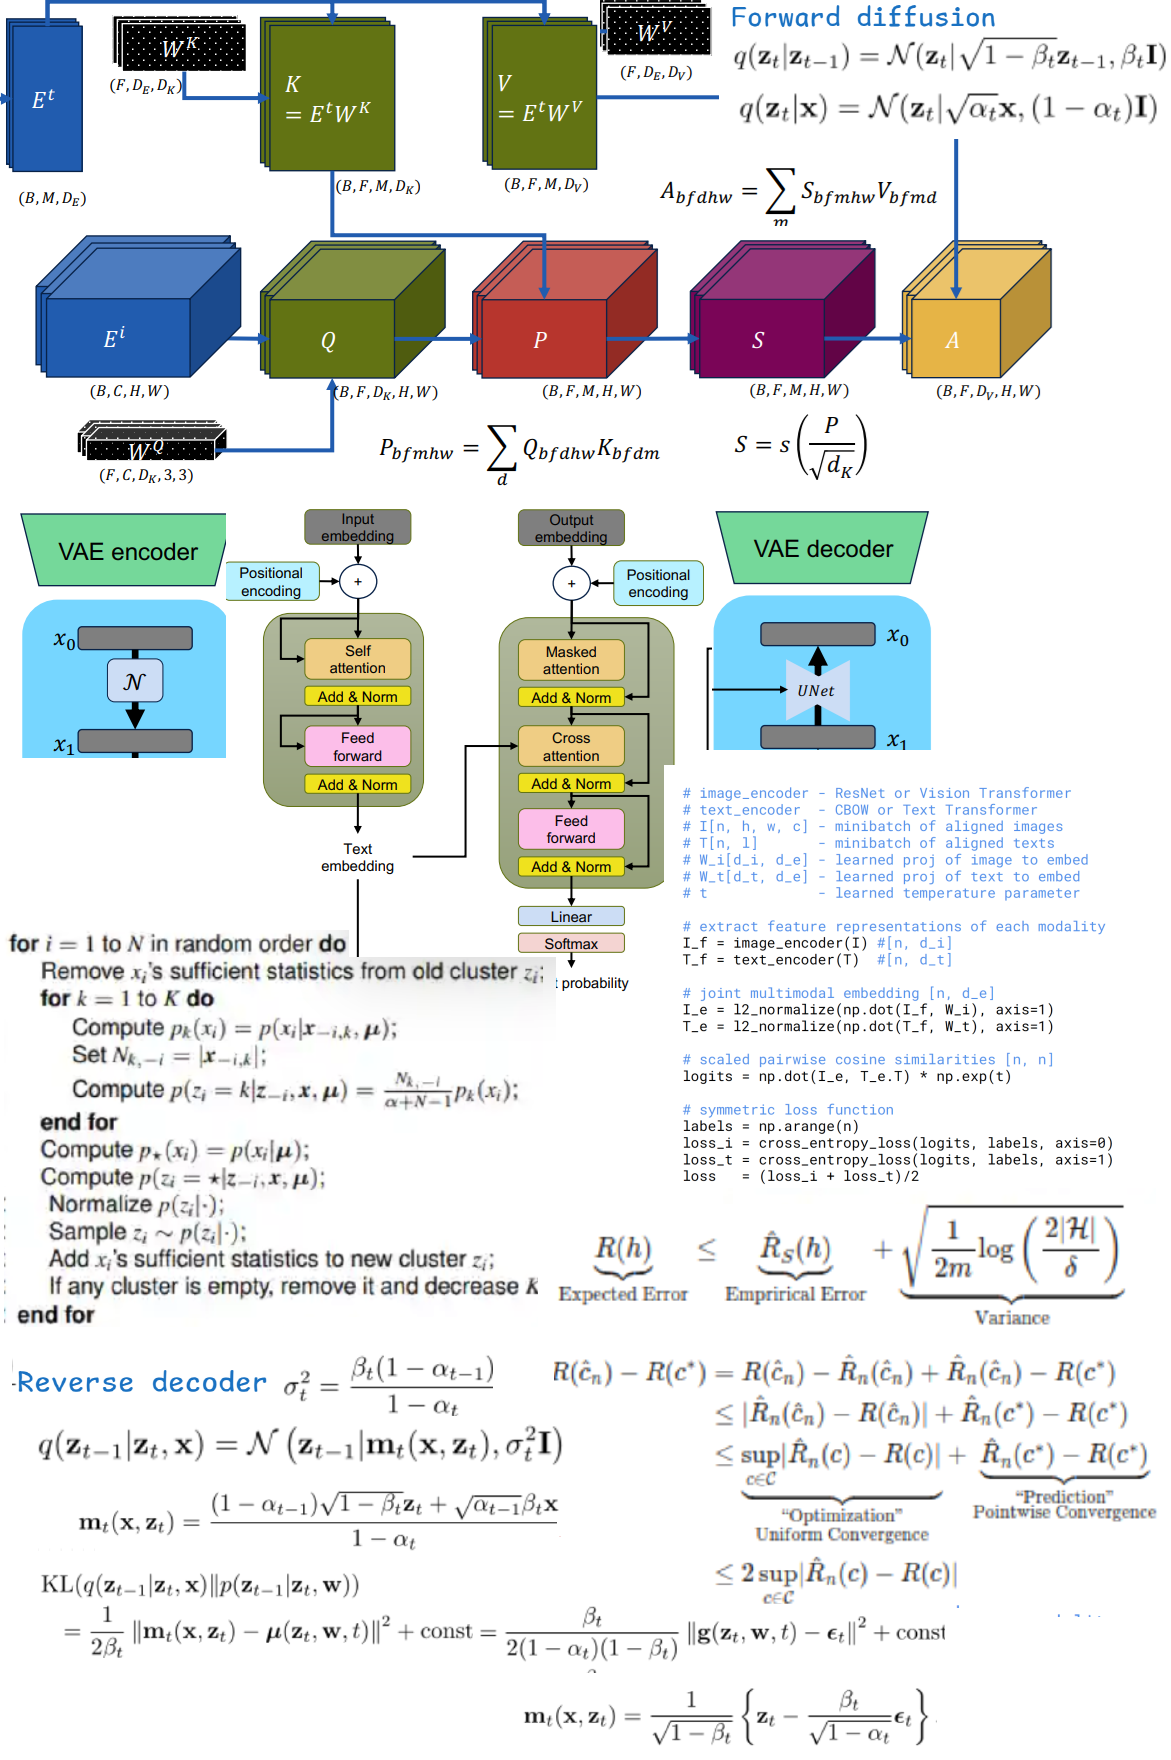
\includegraphics[scale=0.27]{AAA}
\end{multicols*}
\end{document}